\begin{figure}[htbp]
    \centering
    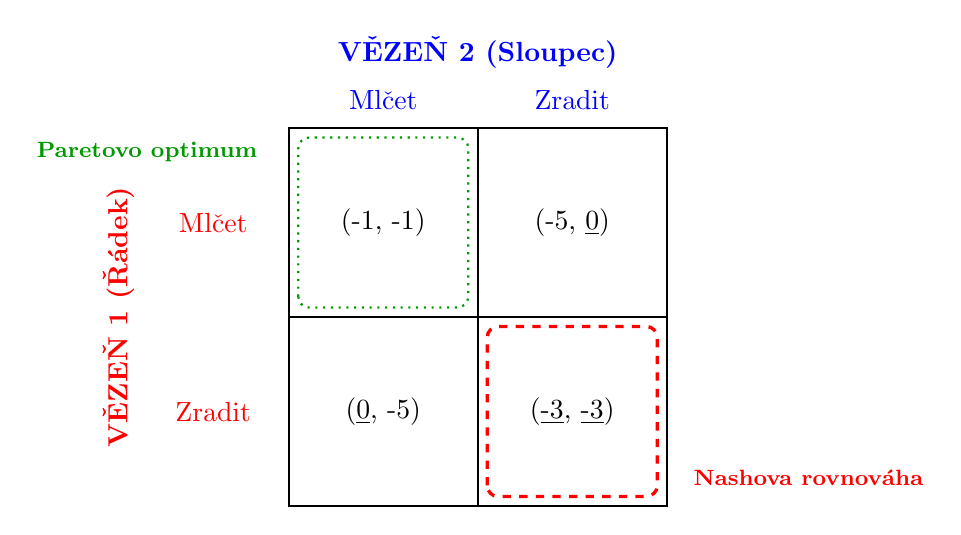
\begin{tikzpicture}[scale=1.2]
        % Mřížka matice
        \draw[thick] (0,0) rectangle (4,4);
        \draw[thick] (2,0) -- (2,4);
        \draw[thick] (0,2) -- (4,2);

        % Hlavičky
        \node[blue, font=\bfseries] at (2, 4.8) {VĚZEŇ 2 (Sloupec)};
        \node[blue] at (1, 4.3) {Mlčet};
        \node[blue] at (3, 4.3) {Zradit};

        \node[red, font=\bfseries, rotate=90] at (-1.8, 2) {VĚZEŇ 1 (Řádek)};
        \node[red] at (-0.8, 3) {Mlčet};
        \node[red] at (-0.8, 1) {Zradit};

        % Výplaty (Záporná čísla znamenají roky ve vězení)
        % V1 mlčí, V2 mlčí
        \node at (1, 3) {(-1, -1)};
        
        % V1 mlčí, V2 zradí -> V1 dostane 5 let, V2 jde na svobodu (0) -> Podtrhneme 0
        \node at (3, 3) {(-5, \underline{0})};
        
        % V1 zradí, V2 mlčí -> V1 jde na svobodu (0), V2 dostane 5 let -> Podtrhneme 0
        \node at (1, 1) {(\underline{0}, -5)};
        
        % Oba zradí -> Oba dostanou 3 roky. Podtrhneme obě výplaty -> Nashova rovnováha!
        \node at (3, 1) {(\underline{-3}, \underline{-3})};

        % Zvýraznění Nashovy rovnováhy
        \draw[red, very thick, dashed, rounded corners] (2.1, 0.1) rectangle (3.9, 1.9);
        \node[red, font=\footnotesize\bfseries] at (5.5, 0.3) {Nashova rovnováha};
        
        % Zvýraznění Paretova optima (Logicky lepší stav, ale matematicky nestabilní)
        \draw[green!60!black, thick, dotted, rounded corners] (0.1, 2.1) rectangle (1.9, 3.9);
        \node[green!60!black, font=\footnotesize\bfseries] at (-1.5, 3.75) {Paretovo optimum};
    \end{tikzpicture}
    \caption{Řešení Vězňova dilematu. Podtržené hodnoty označují nejlepší odpověď hráče na tah soupeře. Červená buňka se dvěma podtržítky je stabilní Nashova rovnováha.}
\end{figure}